\documentclass[a4paper]{article}

%%%%%%%%%%%%%%%%%%%%%%%%%%%%%%%%%%%%%%%%%%%%%%%%%%%%%%%%%%%%%%%%%%%%%%%%%%%%
% Some common includes. Add additional includes you need.
%%%%%%%%%%%%%%%%%%%%%%%%%%%%%%%%%%%%%%%%%%%%%%%%%%%%%%%%%%%%%%%%%%%%%%%%%%%%
\RequirePackage{ngerman}
\RequirePackage[utf8]{inputenc}
\RequirePackage[T1]{fontenc}
\RequirePackage[margin=23mm,bottom=30mm]{geometry}
\RequirePackage{graphicx}
\RequirePackage{amsmath,amsfonts,amssymb,amsthm}
\input kvmacros
\usepackage[dvipsnames]{xcolor}
\usepackage{graphicx} 
\usepackage{tikz}
\usepackage{tkz-graph}
\usepackage{arydshln}
\usepackage{multirow}
\usetikzlibrary{calc}%
\usepackage{ stmaryrd } %lightning in mathmode
\usepackage{ wasysym } %average/diameter
%%%%%%%%%%%%%%%%%%%%%%%%%%%%%%%%%%%%%%%%%%%%%%%%%%%%%%%%%%%%%%%%%%%%%%%%%%%%
% Defines for mathematical notation. Add additional defines as needed.
%%%%%%%%%%%%%%%%%%%%%%%%%%%%%%%%%%%%%%%%%%%%%%%%%%%%%%%%%%%%%%%%%%%%%%%%%%%%
\def\O{\mathcal{O}}
\def\sort{\mathrm{sort}}
\def\scan{\mathrm{scan}}
\def\dist{\mathrm{dist}}
\def\N{\mathcal{N}}
\def\P{\mathcal{P}}
%%%%%%%%%%%%%%%%%%%%%%%%%%%%%%%%%%%%%%%%%%%%%%%%%%%%%%%%%%%%%%%%%%%%%%%%%%%%
% Definition of the assignment header
%%%%%%%%%%%%%%%%%%%%%%%%%%%%%%%%%%%%%%%%%%%%%%%%%%%%%%%%%%%%%%%%%%%%%%%%%%%%
%%%%%%%%%%%%%%%%%%%%%%%%%%%%%%%%%%%%%%%%%%%%%%%%%%%%%%%%%%%%%%%%%%%%%%%%%%%%
% Do not edit this header
%%%%%%%%%%%%%%%%%%%%%%%%%%%%%%%%%%%%%%%%%%%%%%%%%%%%%%%%%%%%%%%%%%%%%%%%%%%%
% These commands are used to generate the header
\newcommand{\lecture}[1]{%
  \def\uebcslecture{#1}%
}

\newcommand{\semester}[1]{%
  \def\uebcssemester{#1}%
}


\newcommand{\student}[3]{%
  \def\uebcsstdname{#1}%
  \def\uebcsstdid{#2}%
  \def\uebcsstdgroup{#3}%
}
\newcommand{\studentshort}[2]{%
  \def\name2{#1}%
  \def\id2{#2}%
}

\newcommand{\assignment}[1]{%
  \def\uebcsnr{#1}%
}

% The different texts are defined for English and German
\DeclareOption{german}
{
% i18n: deutsch
\def\uebcsassignment{\"Ubung }
\def\uebcsexercise{Aufgabe}
\def\uebcsgroup{Gruppe}
\def\uebcsmatnr{Mat.-Nr.}
}

\DeclareOption{english}
{
% i18n: english
\def\uebcsassignment{Assignment}
\def\uebcsexercise{Exercise}
\def\uebcsgroup{Group}
\def\uebcsmatnr{Student ID number}
}


% This environment sets the spaces around the exercises
\newenvironment{exercise}[1]{{%
\vspace{3ex}%
\large%
\noindent\textbf{\uebcsexercise\ \uebcsnr.#1} %
\par\vspace{1ex}%
}}{}

% A small helper box
\def\debugbox#1{%
\fboxrule1pt%
\fboxsep-1pt%
\fbox{#1}%
}
\def\debugbox#1{#1}

% Definition of the assignment header
\def\uebcsuebungheader{{
\parskip3mm
\parbox{\textwidth}{
\debugbox{
\parbox[t]{10cm}{
\vskip0pt
\hspace{-10mm}
\huge\uebcslecture
\vskip3mm
\hspace{-10mm}
\Large\uebcssemester 
\vskip3mm
\hspace{-10mm}
\huge \uebcsassignment \uebcsnr
}
}
\hfill
\debugbox{
\parbox[t]{62mm}{
\raggedleft
\vskip0pt
\Large \uebcsstdname
\vskip2mm
\Large \uebcsmatnr\ \uebcsstdid
\vskip2mm
%\Large \uebcsgroup\ \uebcsstdgroup
%\vskip1mm 
\hrule
\vskip2mm 
\Large \name2 
\vskip2mm 
\Large \uebcsmatnr\ \id2
}
}
}
\vskip5mm
\hrule 
\vskip3ex
}}

% Add header to the beginning of the document
\AtBeginDocument{\uebcsuebungheader}

%%%%%%%%%%%%%%%%%%%%%%%%%%%%%%%%%%%%%%%%%%%%%%%%%%%%%%%%%%%%%%%%%%%%%%%%%%%%
%%%%%%%%%%%%%%%%%%%%%%%%%%%%%%%%%%%%%%%%%%%%%%%%%%%%%%%%%%%%%%%%%%%%%%%%%%%%

% Set option "german" or "english", depending on what language the
% default texts should be in.
\ExecuteOptions{german}
\ProcessOptions

% Enter the lecture name and semester
\lecture{Human Computer Interaction}
\semester{WS 18/19}


% Enter your data: Name, Matrikelnummer (student ID number) and group
\student{Elisabeth Fughe }{5263769}{lol}
\studentshort{Amer El-Ankah} {5750818}
% Which assignment is this?
\assignment{2}

\usepackage{hyperref}

\begin{document}
\[\begin{exercise}{1 - Barrierefreiheit - Farbe} 
Bei der Auswahl der Farben für das Light und Dark Theme sollten folgende Sehschwächen berücksichtigt werden:
Tritanomalie (Blauschwäche)
Deuteranopie (Grünblindheit)
Presbyopie (Altersweitsichtigkeit)

Aus diesem Grund war es besonders beim Dark Theme von großer Bedeutung die richtigen Farben zu wählen. 
Wir haben uns an dieser Stelle dazu entschieden, dunkle Grauabstufungen bzw. Schwarz für die Hintergründe zu verwenden. Diese Grau- bzw. Schwarztöne werden im Vergleich zu dunklen Blautönen durch die Tritanomalie oder Deuteranopie kaum verändert und somit bleiben die Farben auch für Menschen mit diesen Sehschwächen fast unverändert (Bsp. Siehe unten). Zudem haben wir uns dafür entschieden eine weiße Schrift auf diesem Hintergrund zu verwenden, sodass auch für Menschen die an Altersweitsichtigkeit leiden die Seite gut lesbar bleibt, da sich die Schrift eindeutig von den Hintergrund abhebt. Auch die Bücherthumbnails haben einen weisen Hintergrund, damit dieser sich im Dark Theme gut vom Rest der Website abhebt und dadurch nochmal ein Fokus auf diese geworfen wird.

Das Light Theme ist in den Farben unverändert, da diese bereits alle oben genannten Ansprüche erfüllt haben. An dieser Stelle haben wir davon abgesehen Hintergründe schwarz bzw grau zu gestalten um einen Fokus auf diese zu werfen, da das eher ungewöhnlich für Light Themes ist.
Die Farben des Light Themes sind ebenfalls so gewählt, dass Tritanomalie oder Deuteranopie keinen Einfluss auf die Lesbarkeit der Website hat, wobei hier klar ist, dass sich die Farben für den Betrachten mit einer dieser Sehschwächen verändert, da helle Töne einfach mehr Blau bzw. Grünspektren besitzen.


Farbwahl Dark Theme
Dark-grey (Navigation Bar): #333132
Light-grey: #bcbbbb
Default-font-color: #000000

Farbwahl Light Theme
Dark-grey (Navigation Bar): #000000
Light-grey: #0E0F10
Default-font-color: #ffffff\\\\

\begin{Large}
\textbf{Tritanomalie Light Theme:}
\end{Large}\\\\
\begin{center}
 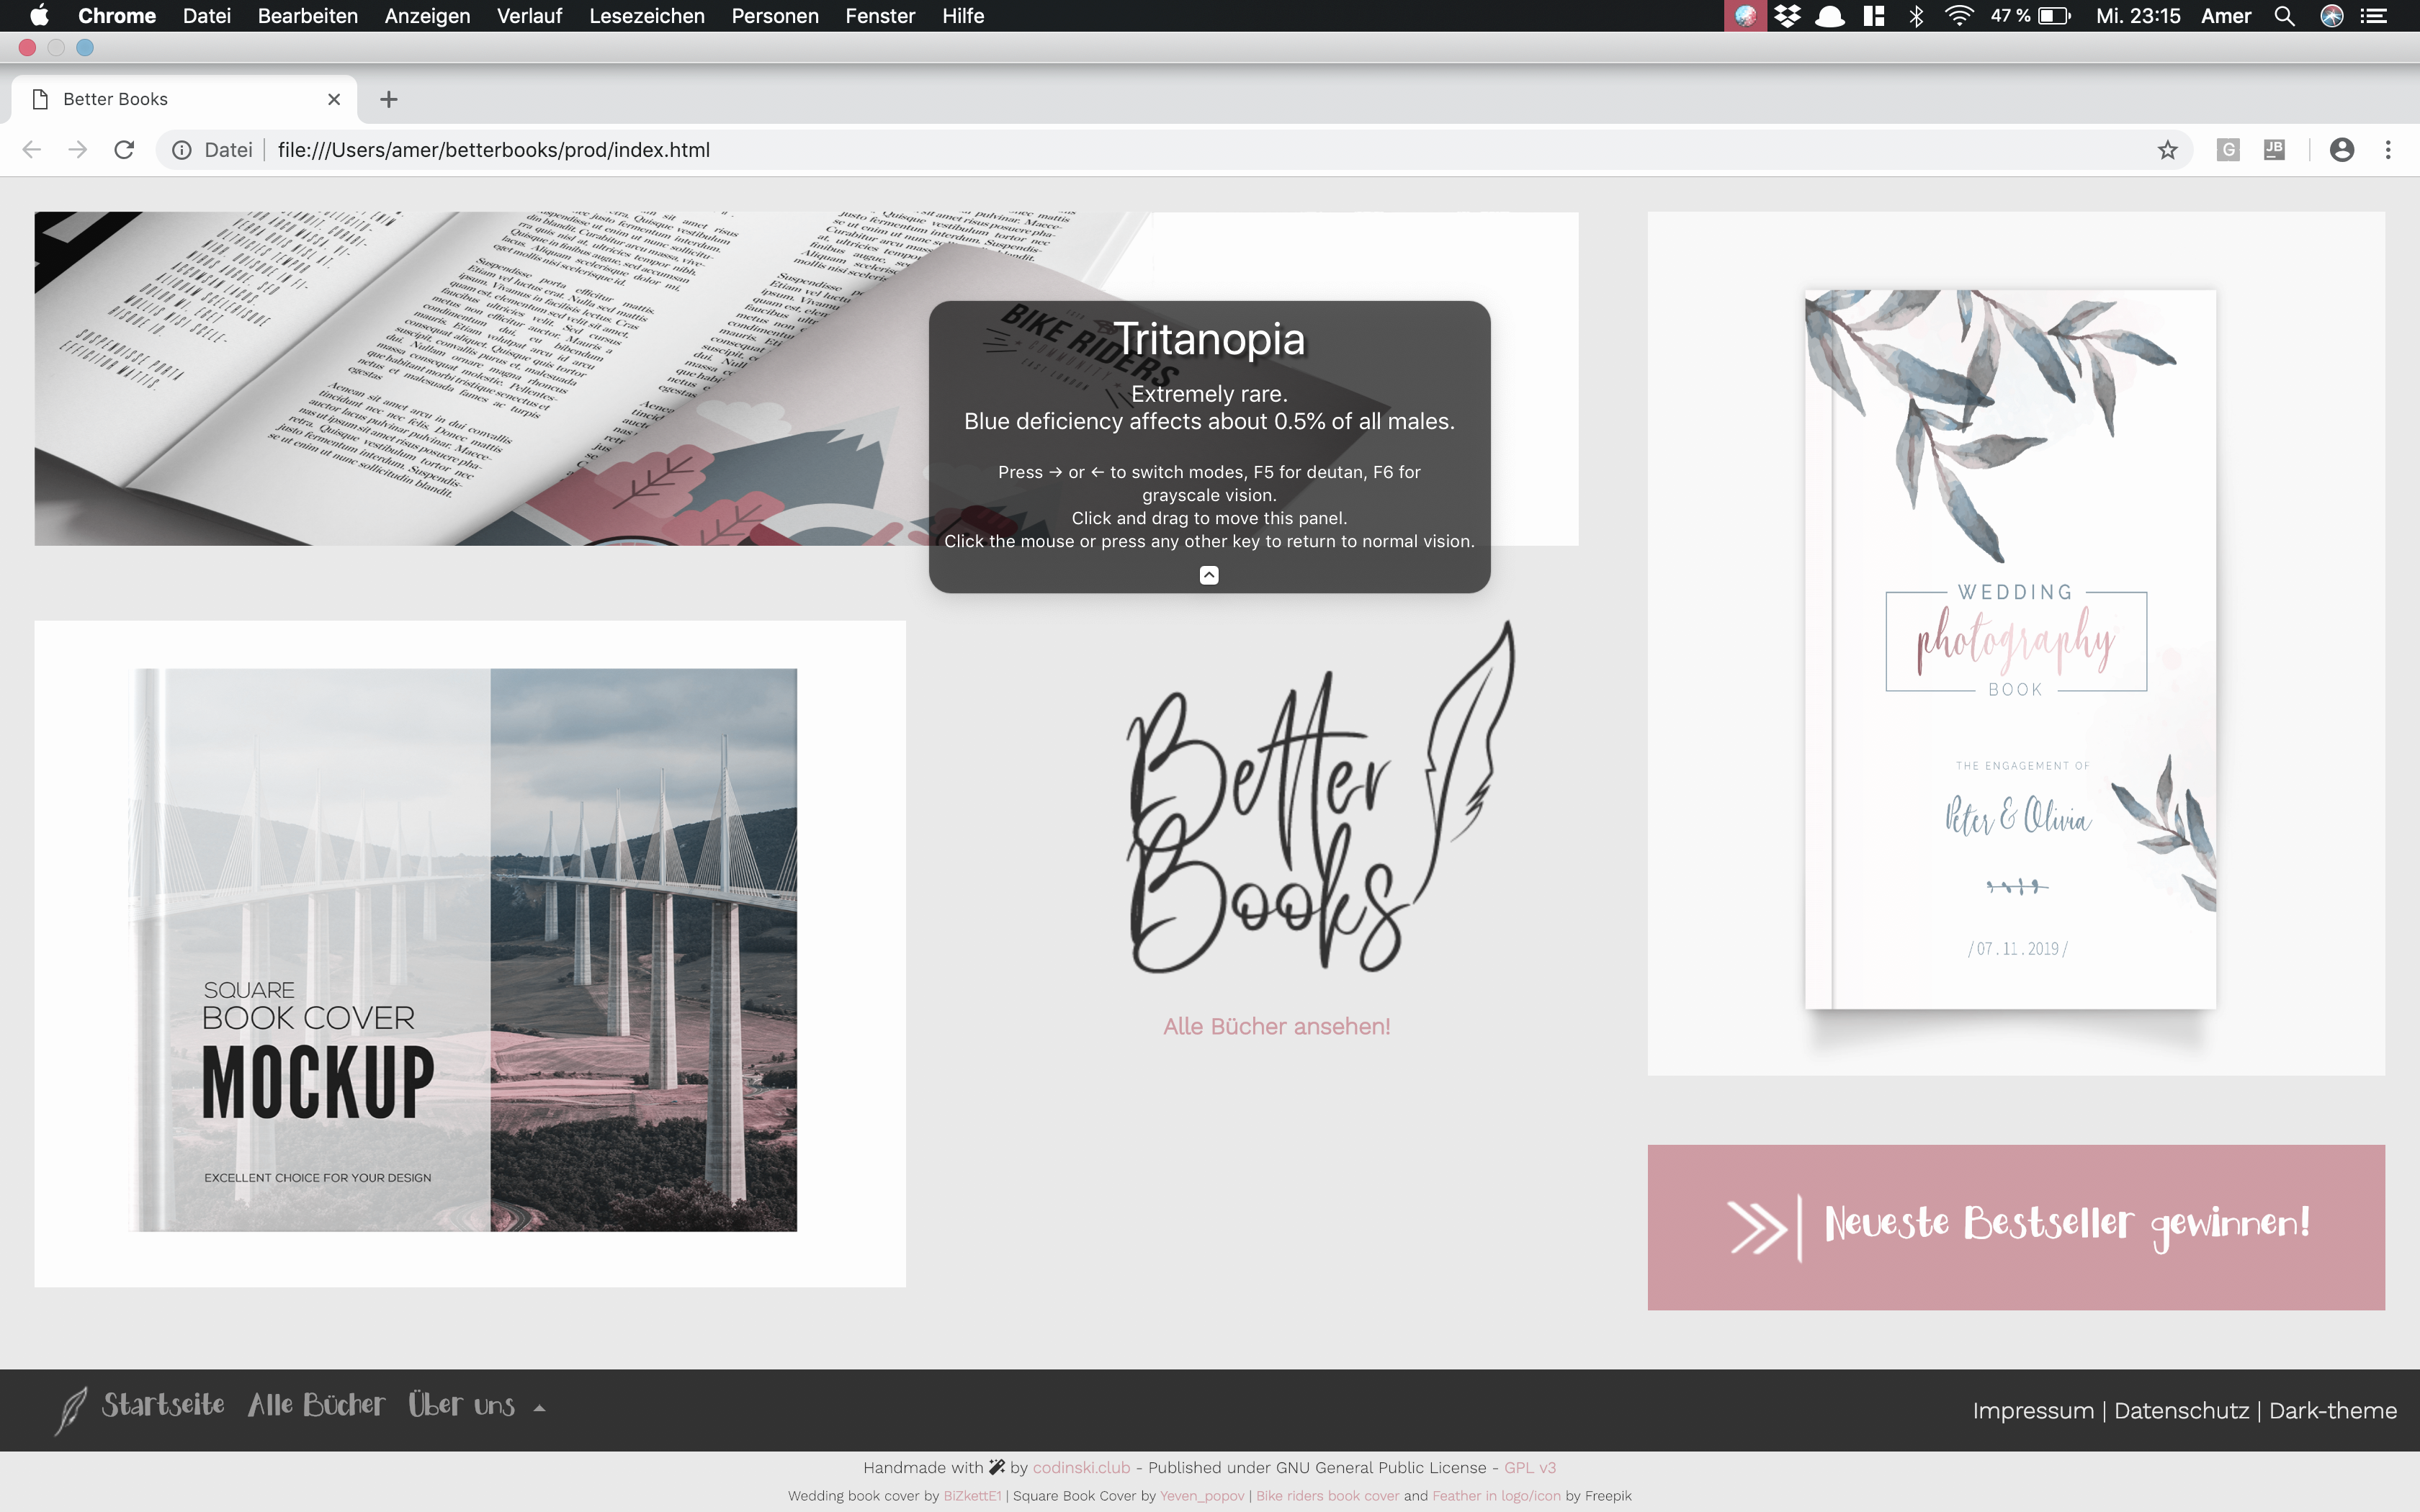
\includegraphics[scale=0.5]{../6_bookstore_main_tritanomalie_light.png}
 \end{center}
\begin{Large}
\textbf{Tritanomalie Dark Theme:}
\end{Large}\\\\
\begin{center}
 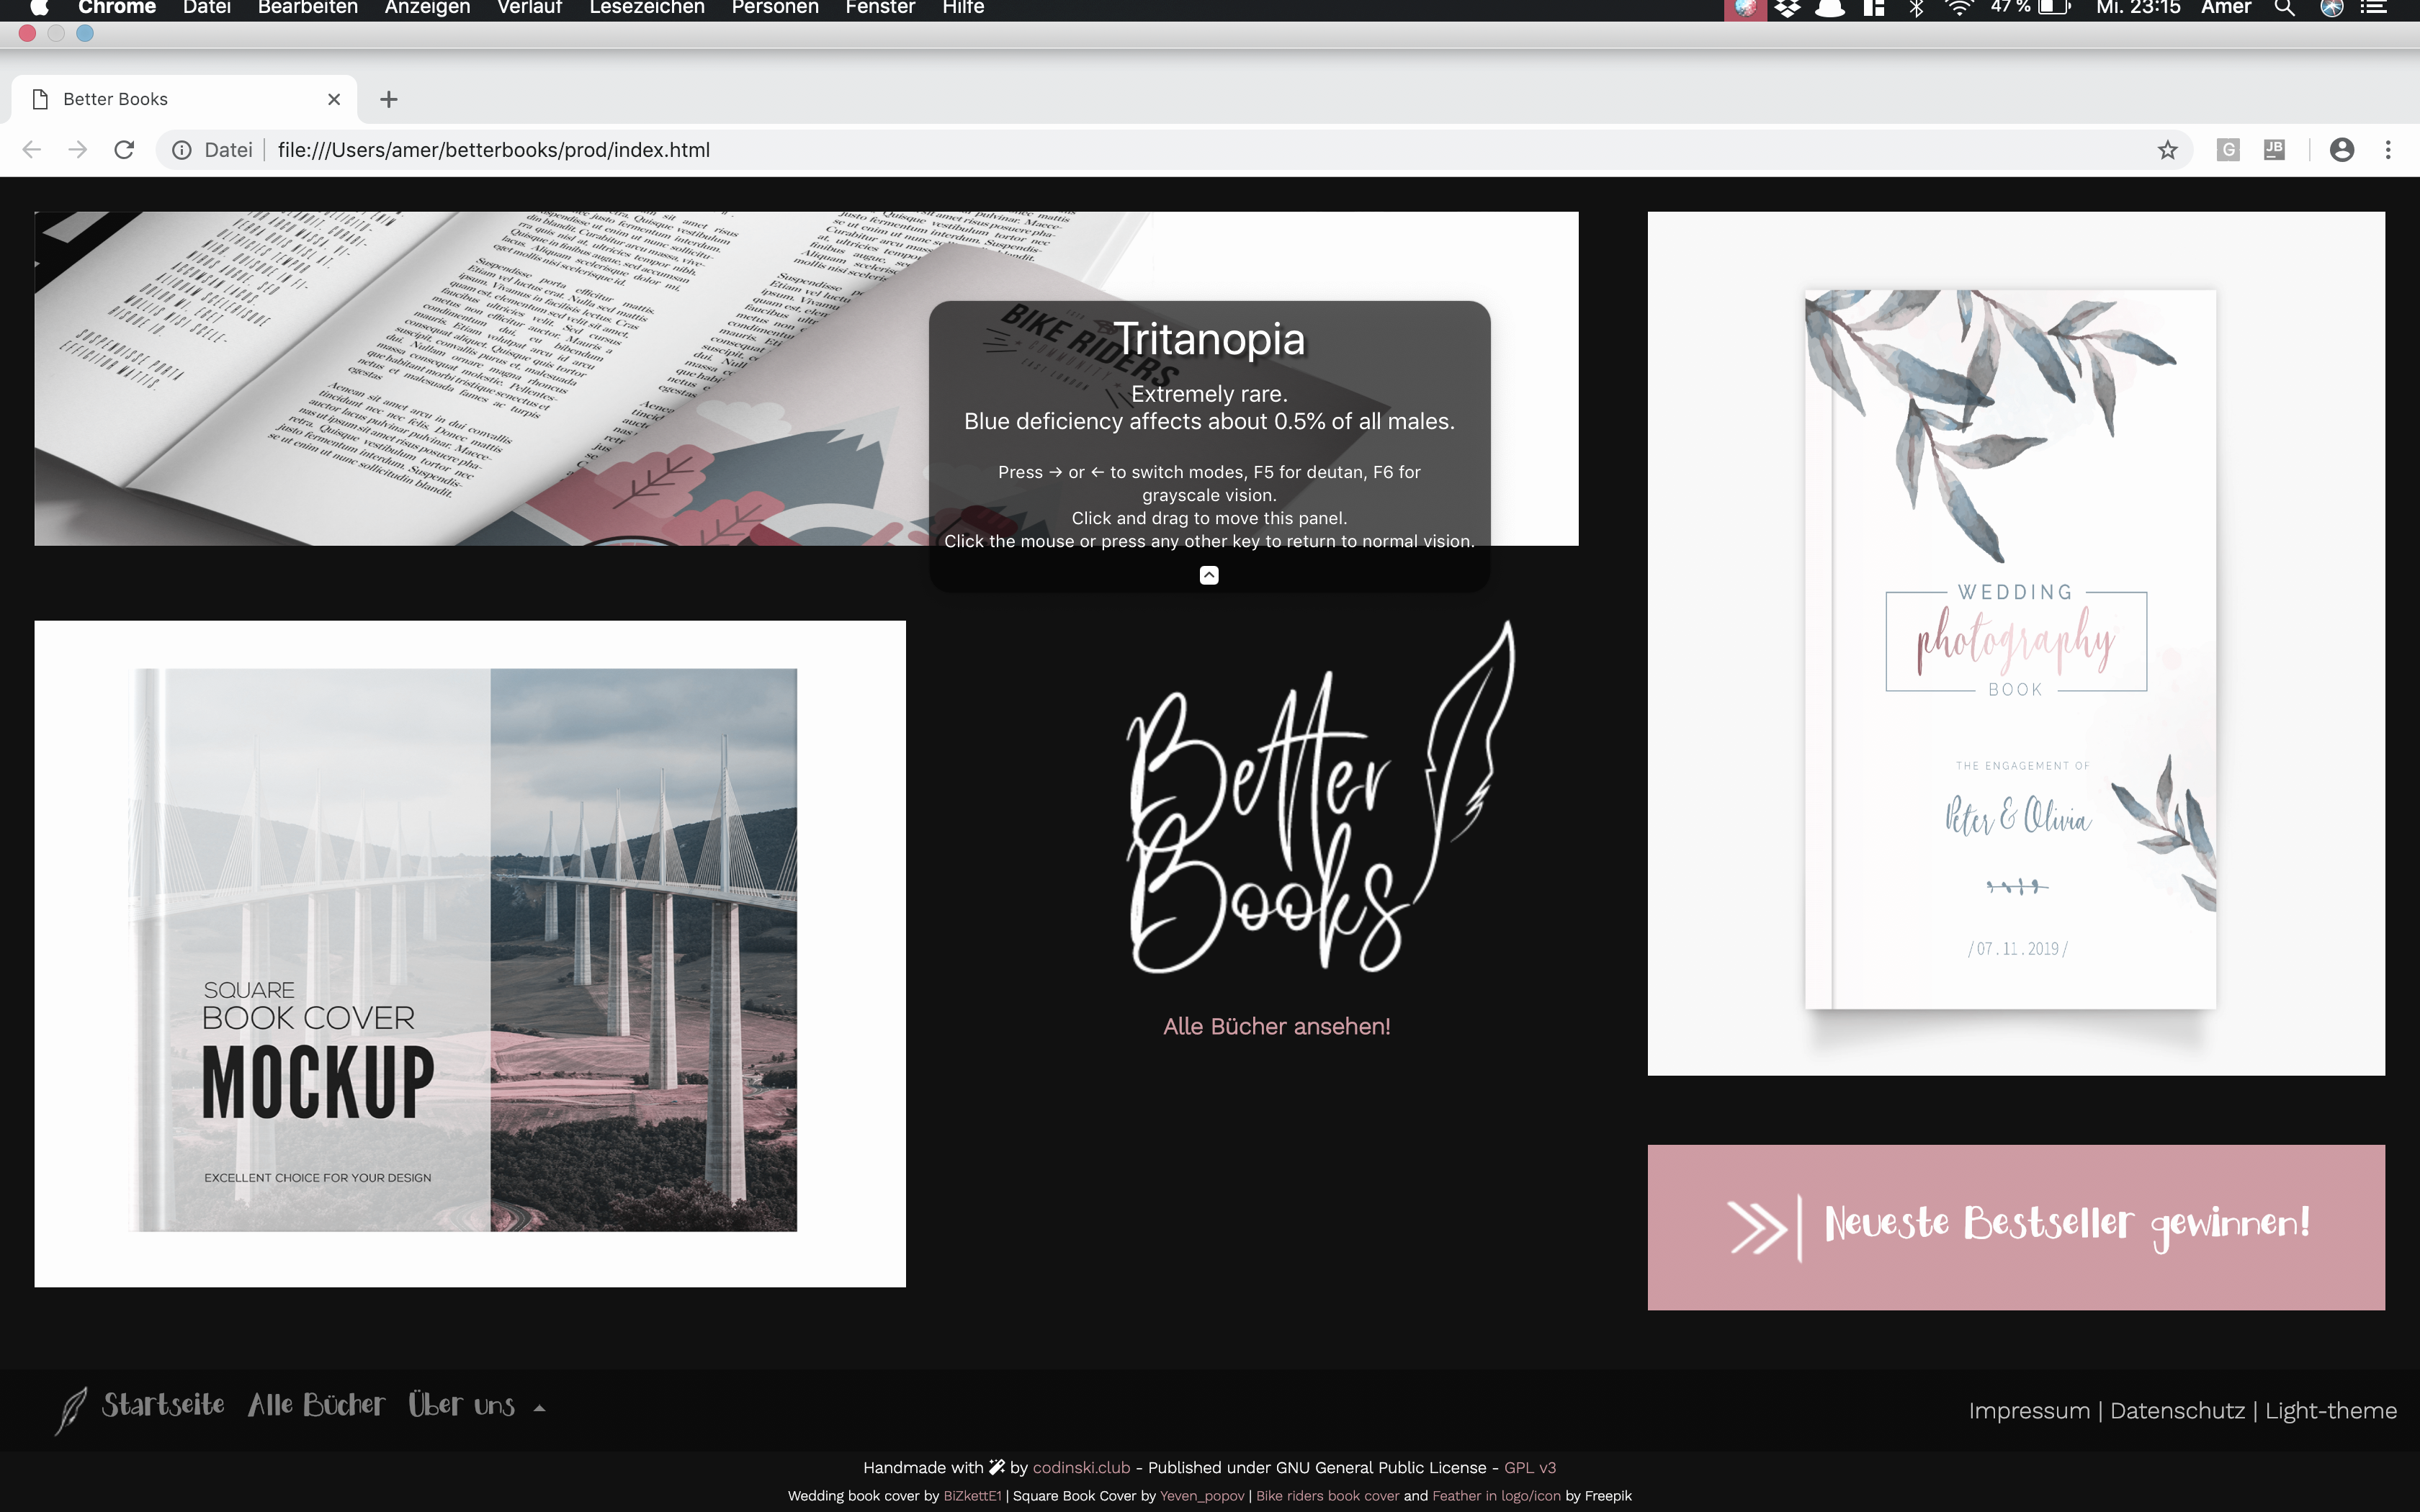
\includegraphics[scale=0.5]{../7_bookstore_main_tritanomalie_dark.png}
 \end{center}
\begin{Large}
\textbf{Deuteranopie Light Theme:}
\end{Large}\\\\
\begin{center}
 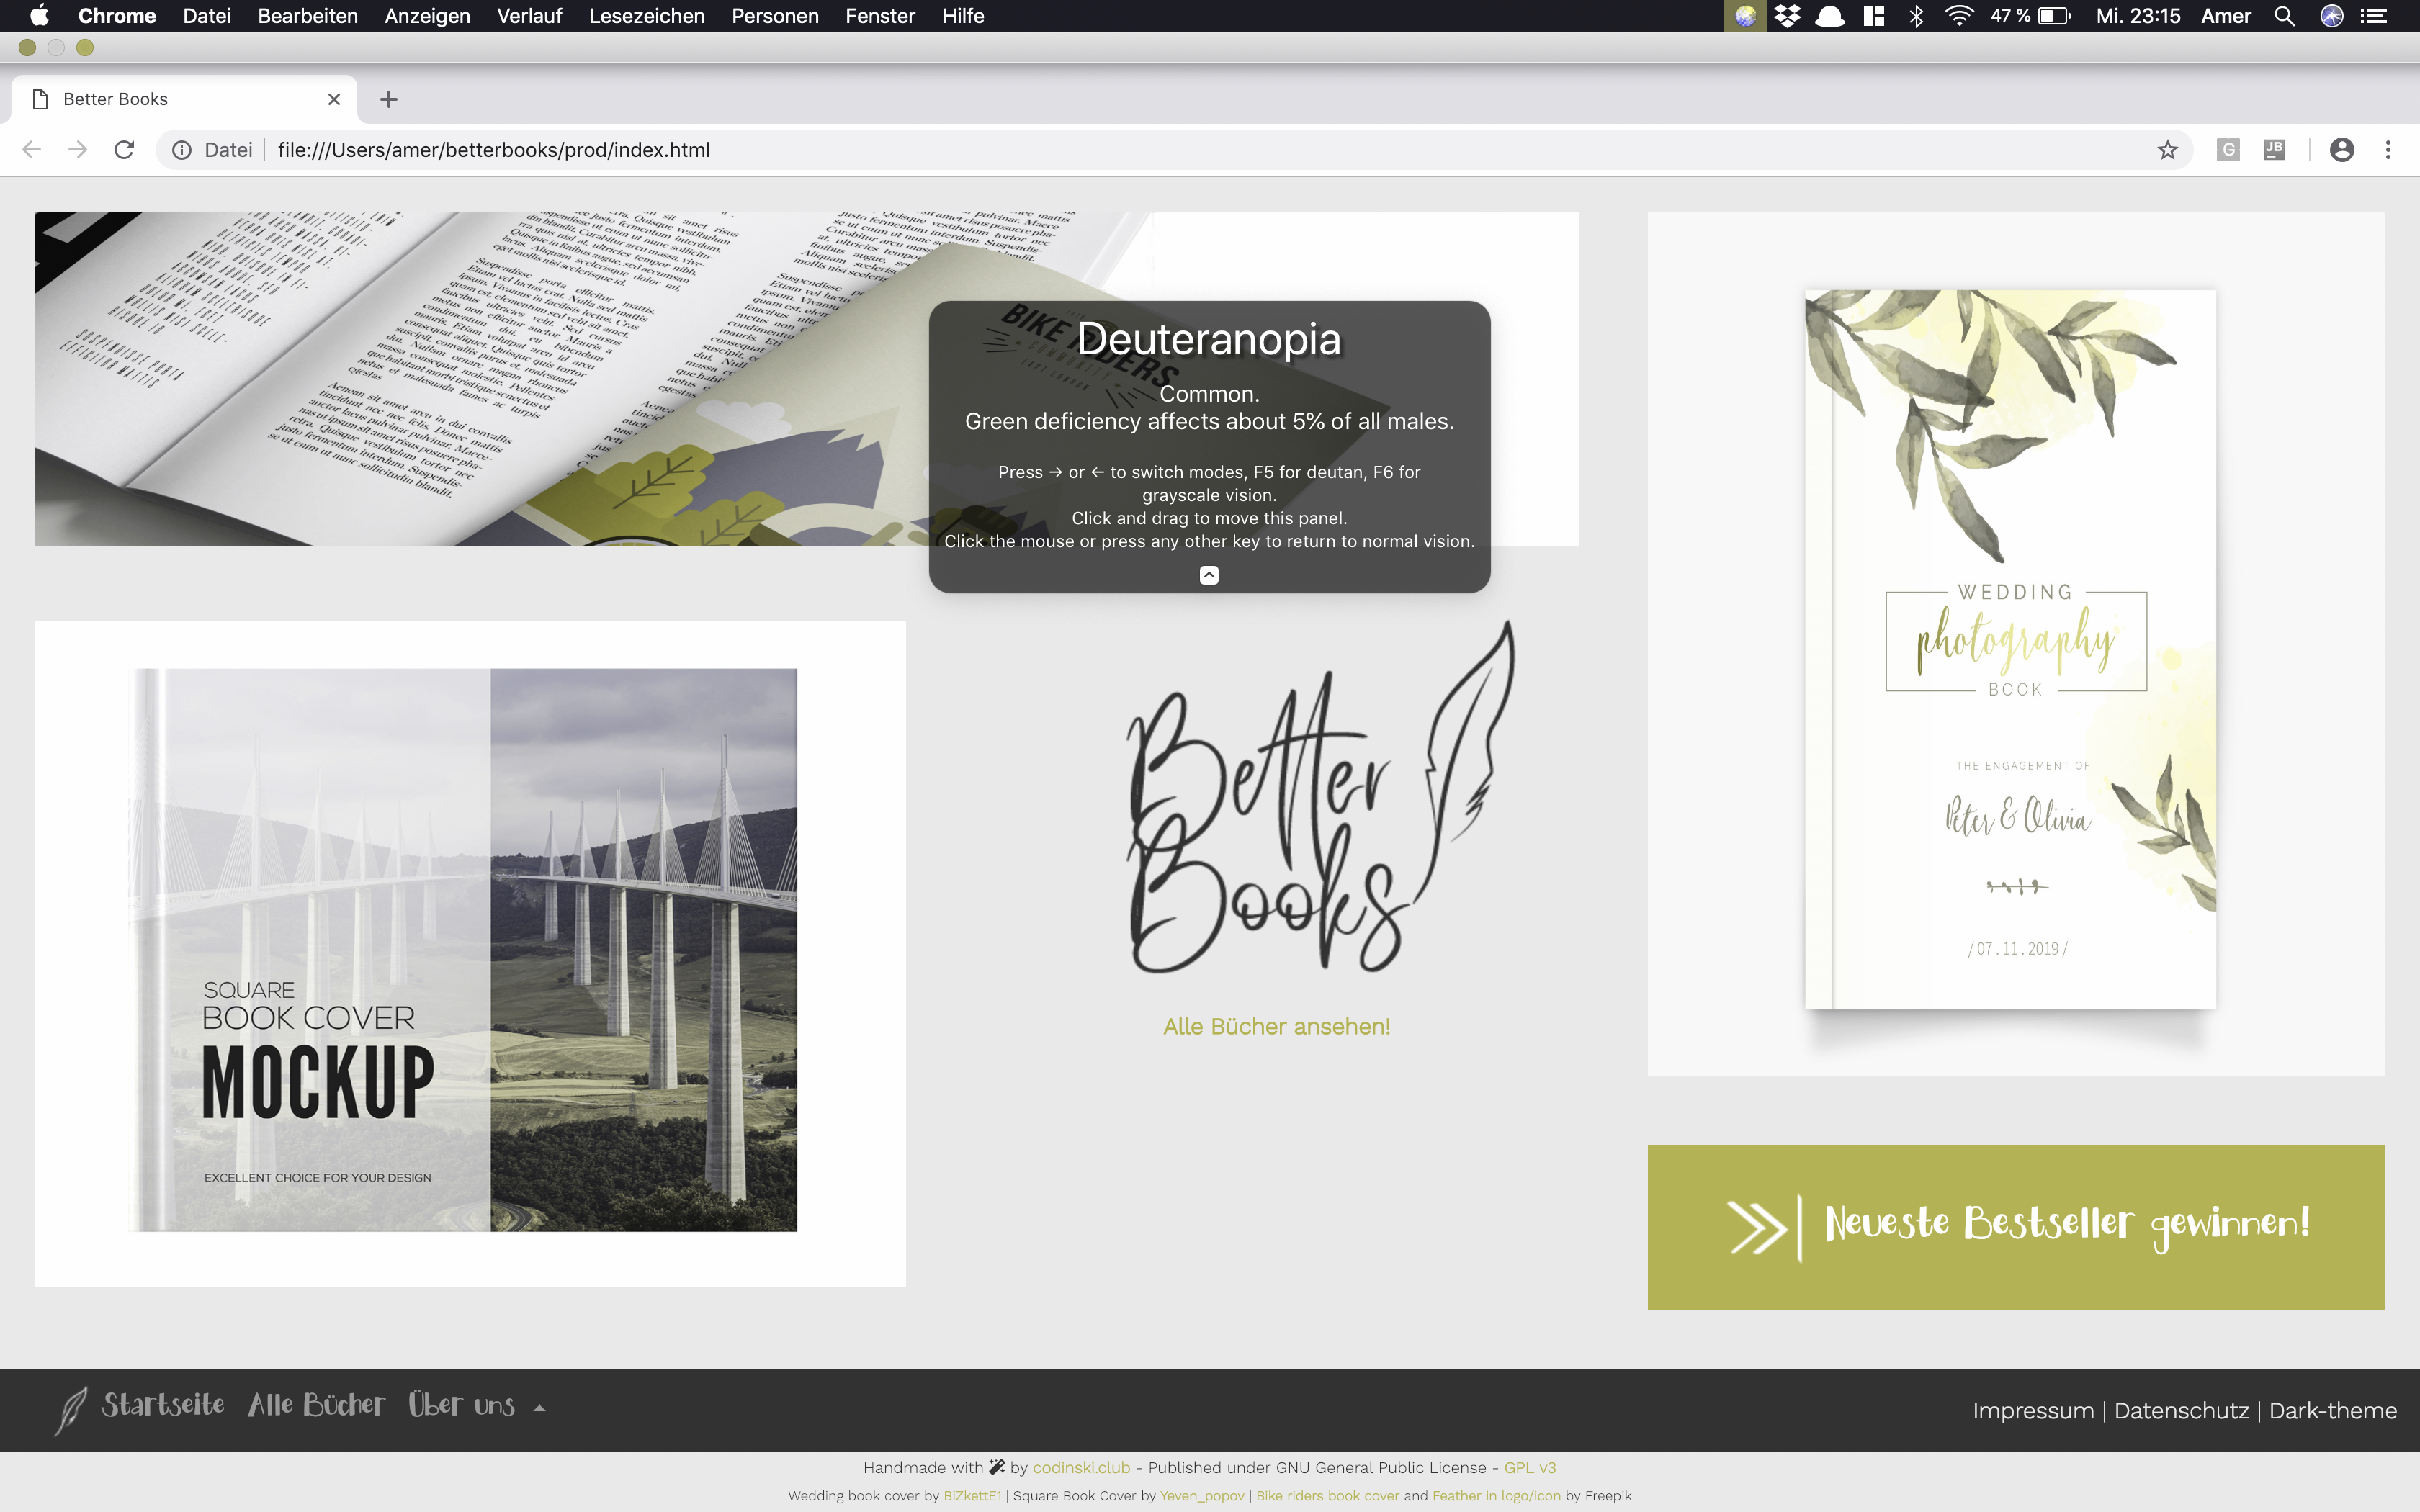
\includegraphics[scale=0.5]{../8_bookstore_main_deuteranopie_light.png}
 \end{center}
\begin{Large}
\textbf{Deuteranopie Dark Theme:}
\end{Large}\\\\
\begin{center}
 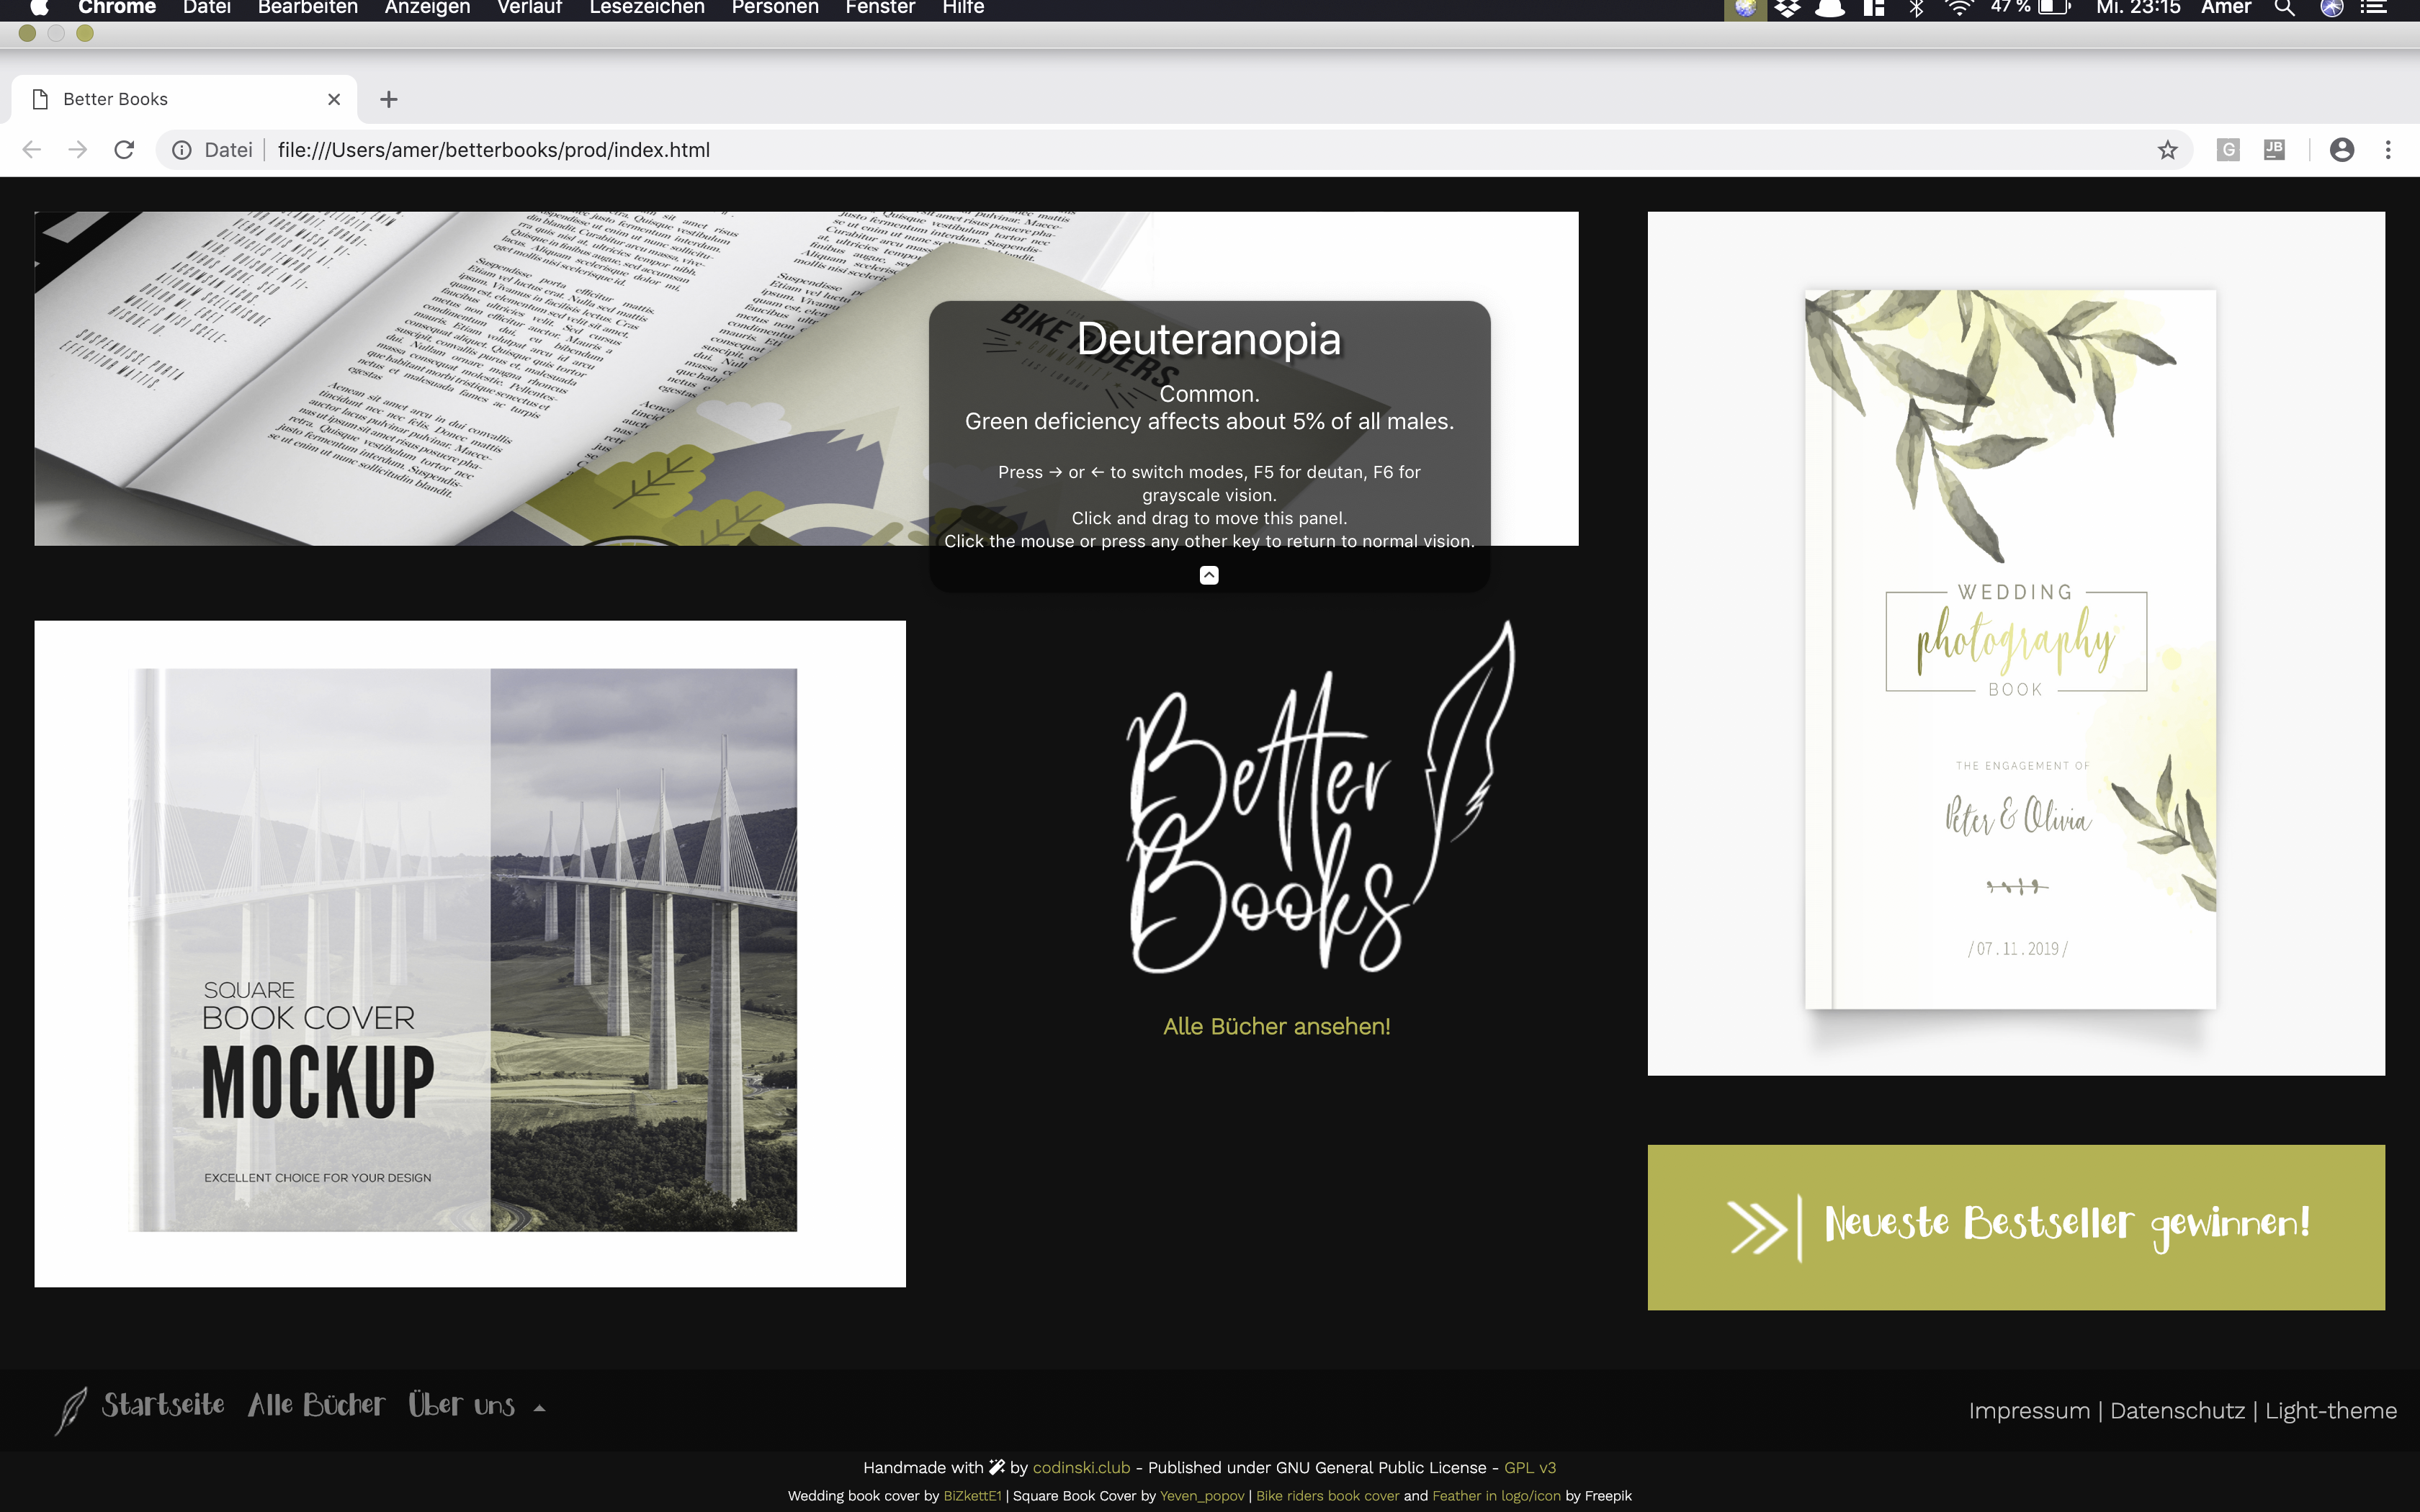
\includegraphics[scale=0.5]{../9_bookstore_main_deuteranopie_dark.png}
 \end{center}



\end{exercise}

\]
\end{document}